% preamble.tex provides all settings and packages needed for a well
% structured report. For full description and documentation please visit
% https://CTAN.org/.

% Best practice:
% Use this together with the main-tfy.tex file. Put additional packages and
% commands at the bottom of this file or temporary packages in the main-tfy.tex
% file. Write each section in a separate file and include them in the
% main-tfy.tex file using \include{foo.tex} or \input{bar.tex}

% Contributors
% Filip Edström, Joar Svartholm - F 14, 14/5-2018

% ----------------------------- Document settings -----------------------------

\documentclass[a4paper,11pt]{article}
% Description: Initializes a format class from a .cls file.
% Note: Some built in examples are: article, report, book, IEEEtran, beamer. For two column article add 'twocolumn' as argument or use class IEEEtran
% Usage:

% ----------------------------- Input and Output ------------------------------

\usepackage[utf8]{inputenc}
% Description: Trans­lates var­i­ous stan­dard and other in­put en­cod­ings into a ‘LATEX in­ter­nal lan­guage’. Enables usage of Swedish letters.
% Note:
% Usage:


\usepackage[T1]{fontenc}
% Description: Al­lows the user to se­lect font en­cod­ings, and for each en­cod­ing pro­vides an in­ter­face to ‘font-en­cod­ing-spe­cific’ com­mands for each font.
% Note:
% Usage:


\usepackage[english]{babel}
% Description: Man­ages cul­tur­ally-de­ter­mined ty­po­graph­i­cal (and other) rules, and hy­phen­ation pat­terns for a wide range of lan­guages.
% Note:
% Usage:


\usepackage{gensymb}
% Description: Pro­vides generic com­mands \de­gree, \cel­sius, \pert­hou­sand, \mi­cro and \ohm which work both in text and maths mode.
% Note:
% Usage:


\usepackage{color}
% Description: Pro­vides both fore­ground (text, rules, etc.) and back­ground colour man­age­ment; it uses the de­vice driver con­fig­u­ra­tion mech­a­nisms of the graph­ics pack­age to de­ter­mine how to con­trol its oup­tut.
% Note:
% Usage:

% -------------------------------- Page Layout --------------------------------

\usepackage{geometry}
% Description: The pack­age pro­vides an easy and flex­i­ble user in­ter­face to cus­tomize page lay­out, im­ple­ment­ing auto-cen­ter­ing and auto-bal­anc­ing mech­a­nisms so that the users have only to give the least de­scrip­tion for the page lay­out. Add additional arguments for change of margins.
% Note: Possible usage \usepackage[margin=3cm,bottom=4cm,nohead]{geometry}


\usepackage{fancyhdr}
% Description: Pro­vides ex­ten­sive fa­cil­i­ties, both for con­struct­ing head­ers and foot­ers, and for con­trol­ling their use (for ex­am­ple, at times when LATEX would au­to­mat­i­cally change the head­ing style in use).
% Note:
% Usage:


\usepackage{hyperref}
\hypersetup{
  colorlinks   = true,  %Colours links instead of ugly boxes
  urlcolor     = black, %Colour for external hyperlinks
  linkcolor    = black, %Colour of internal links
  citecolor   = black   %Colour of citations
}
% Description: Used to han­dle cross-ref­er­enc­ing com­mands in LATEX to pro­duce hy­per­text links in the doc­u­ment.
% Note:
% Usage:

% ---------------------------- Image visualization ----------------------------

\usepackage{graphicx,epstopdf,float}
\graphicspath{{./figs/}}
% Description: graphicx makes it possible to include images using \includegraphics[]{}. epstopdf makes it possible to include .eps format images for high quality graphics. float improves figure alignment.
% Note: alignment arguments are 'h'(here), 'H'(here-force), 't'(top),
% 'b'(bottom), '!'(override formatting). Best practice: \begin{figure}[htb],
% put your images in ./figs folder in current directory


\usepackage{subcaption}
% subcaption makes it possible (there are more ways) to create subfigures with  captions.
% Best practice: http://tex.stackexchange.com/questions/91224/placing-two-figures-side-by-side
% Description:
% Note:
% Usage:


\usepackage{wrapfig}
% Al­lows fig­ures or ta­bles to have text wrapped around them.
% Note: Does not work in com­bi­na­tion with list en­vi­ron­ments, but can be used in a par­box or mini­page, and in twocol­umn for­mat. Sup­ports the float pack­age.
% Usage: \begin{wrapfigure}
% Description:
% Note: if you specify a width of zero (0pt), the actual width of the figure will determine the wrapping width.
% Usage:


\usepackage[margin=3ex,font={small,it},labelfont={normal,bf}]{caption}
% Settings for figure captions
% Description:
% Note:
% Usage:

\usepackage{subcaption}
% Description: For subfigure environments
% Note: Better than subfigure and subfig packages since they might not be compatible with hyperref.
% Usage:

% ------------------------------------ Math -----------------------------------
%
\usepackage{amsmath}
% The prin­ci­pal pack­age in the AMS-LATEX dis­tri­bu­tion. It adapts for use in LATEX most of the math­e­mat­i­cal fea­tures found in AMS-TEX; it is highly rec­om­mended as an ad­junct to se­ri­ous math­e­mat­i­cal type­set­ting in LATEX.
% Description:
% Note:
% Usage:

\usepackage{mathtools}
% Math­tools pro­vides a se­ries of pack­ages de­signed to en­hance the ap­pear­ance of doc­u­ments con­tain­ing a lot of math­e­mat­ics.
% Description:
% Note:
% Usage:

\usepackage{amssymb}
% For additional mathematical symbols
% Description:
% Note:
% Usage:

\usepackage{amsfonts}
% An ex­tended set of fonts for use in math­e­mat­ics, in­clud­ing: ex­tra math­e­mat­i­cal sym­bols; black­board bold let­ters (up­per­case only); frak­tur let­ters; sub­script sizes of bold math italic and bold Greek let­ters; sub­script sizes of large sym­bols such as sum and prod­uct; added sizes of the Com­puter Modern small caps font; cyril­lic fonts (from the Univer­sity of Wash­ing­ton); Euler math­e­mat­i­cal fonts.
% Description:
% Note:
% Usage:

% --------------------------------- Miscellaneous -----------------------------
\usepackage{enumerate}
% The pack­age adds an op­tional ar­gu­ment to the enu­mer­ate en­vi­ron­ment which de­ter­mines the style in which the counter is printed.
% Note: for numbered lists
% Usage: \begin{enumerate}
% Description:
% Note:
% Usage:


\usepackage[toc, page]{appendix}
% Description:
% Note:

% --------------------------------- Code snippets -----------------------------
%
\usepackage{listings}
% listing makes it possible to include code as separate files.
% Best practice: Keep your code in a ./code folder and import them using \lstinputlisting{code/foo.m}
% Tip: change code language in \lstset to make the color coding match language
% Note: The color package is required for color coding
% Description:
% Note:
% Settings:
\definecolor{mygreen}{rgb}{0,0.6,0}
\definecolor{mygray}{rgb}{0.5,0.5,0.5}
\definecolor{mymauve}{rgb}{0.58,0,0.82}
\lstset{ %
  backgroundcolor=\color{white},   % choose the background color; you must add \usepackage{color} or \usepackage{xcolor}
  basicstyle=\footnotesize\tt,        % the size of the fonts that are used for the code
  breakatwhitespace=false,         % sets if automatic breaks should only happen at whitespace
  breaklines=true,                 % sets automatic line breaking
  captionpos=t,                    % sets the caption-position to bottom
  commentstyle=\color{mygreen},    % comment style
  deletekeywords={...},            % if you want to delete keywords from the given language
  escapeinside={\%*}{*)},          % if you want to add LaTeX within your code
  extendedchars=true,              % lets you use non-ASCII characters; for 8-bits encodings only, does not work with UTF-8
  frame=single,	                   % adds a frame around the code
  keepspaces=true,                 % keeps spaces in text, useful for keeping indentation of code (possibly needs columns=flexible)
  keywordstyle=\color{blue},       % keyword style
  language=python,                 % the language of the code
  otherkeywords={...},           % if you want to add more keywords to the set
  numbers=left,                    % where to put the line-numbers; possible values are (none, left, right)
  numbersep=5pt,                   % how far the line-numbers are from the code
  numberstyle=\tiny\color{mygray}, % the style that is used for the line-numbers
  rulecolor=\color{black},         % if not set, the frame-color may be changed on line-breaks within not-black text (e.g., comments (green here))
  showspaces=false,                % show spaces everywhere adding particular underscores; it overrides 'showstringspaces'
  showstringspaces=false,          % underline spaces within strings only
  showtabs=false,                  % show tabs within strings adding particular underscores
  stepnumber=2,                    % the step between two line-numbers. If it's 1, each line will be numbered
  stringstyle=\color{mymauve},     % string literal style
  tabsize=2,	                   % sets default tabsize to 2 spaces
  title=\lstname                   % show the filename of files included with \lstinputlisting; also try caption instead of title
}


% ------------------------------ New/renewed commands -------------------------

% Mail as hyperlinks
\newcommand{\mail}[1]{\href{mailto:#1}{\nolinkurl{#1}}}

% This enables referencing to author by myAuthor and referencing to title by myTitle
\let\oldAuthor\author
\renewcommand{\author}[1]{\newcommand{\myAuthor}{#1}\oldAuthor{#1}}
\let\oldTitle\title
\renewcommand{\title}[1]{\newcommand{\myTitle}{#1}\oldTitle{#1}}

% Example of \newcommand:
% Make vector variables in math mode
% Best practice (in math mode): \m{Ax} = \m b
\newcommand{\m}[1]{\mathbf{#1}}


% ------------------- New packages, commands and settings ---------------------
\usepackage{lipsum}

% ----------------------------- Title and Author ------------------------------
  \title{Scientific Report Template}
  \author{
    Göte Johansson - gote1234(\mail{gote1234@student.umu.se}) \and
    Enar Johansson - enrj4321(\mail{enrj4321@student.umu.se})
  }
  \date{\today}

% ------------------------------- Page styles ---------------------------------

% Changes header and footer for the front page.
\fancypagestyle{FirstPageStyle}{
    \headheight 35pt
    \rhead{\small\today}
    \lhead{\small Department of Physics \\ Umeå University}
    \cfoot{Course \\ Supervisor: }
}

% Changes header, footer and indentation (no indent, paragraph skip).
\fancypagestyle{DocumentStyle}{
  \headheight 30pt
  \rhead{\small \myTitle}
  % Ska man verkligen ha author här?!
  \lhead{\small \myAuthor \\ \today}
  \cfoot{\thepage}
  \setlength{\parskip}{5pt plus 1pt minus 1pt}
  \setlength{\parindent}{0pt}
}


% ------------------------------------ Document -------------------------------
\begin{document}

% ----------------------------------- TITLE PAGE ------------------------------
\begin{titlepage}

  \maketitle
  \thispagestyle{FirstPageStyle}

  \begin{abstract}
   \noindent
   This is a suggestion for an updated template for the Engineering Physics programme at Umeå University made by Filip Edström and Joar Svartholm.
  \end{abstract}

\end{titlepage}
% --------------------------------- END TITLE PAGE ----------------------------


% -------------------------------- Table of contents --------------------------
\pagestyle{DocumentStyle}
\tableofcontents
\newpage

% ------------------------------------ Content --------------------------------


\subsection{Appendix style figure}
\begin{figure}[H]
	\centering
	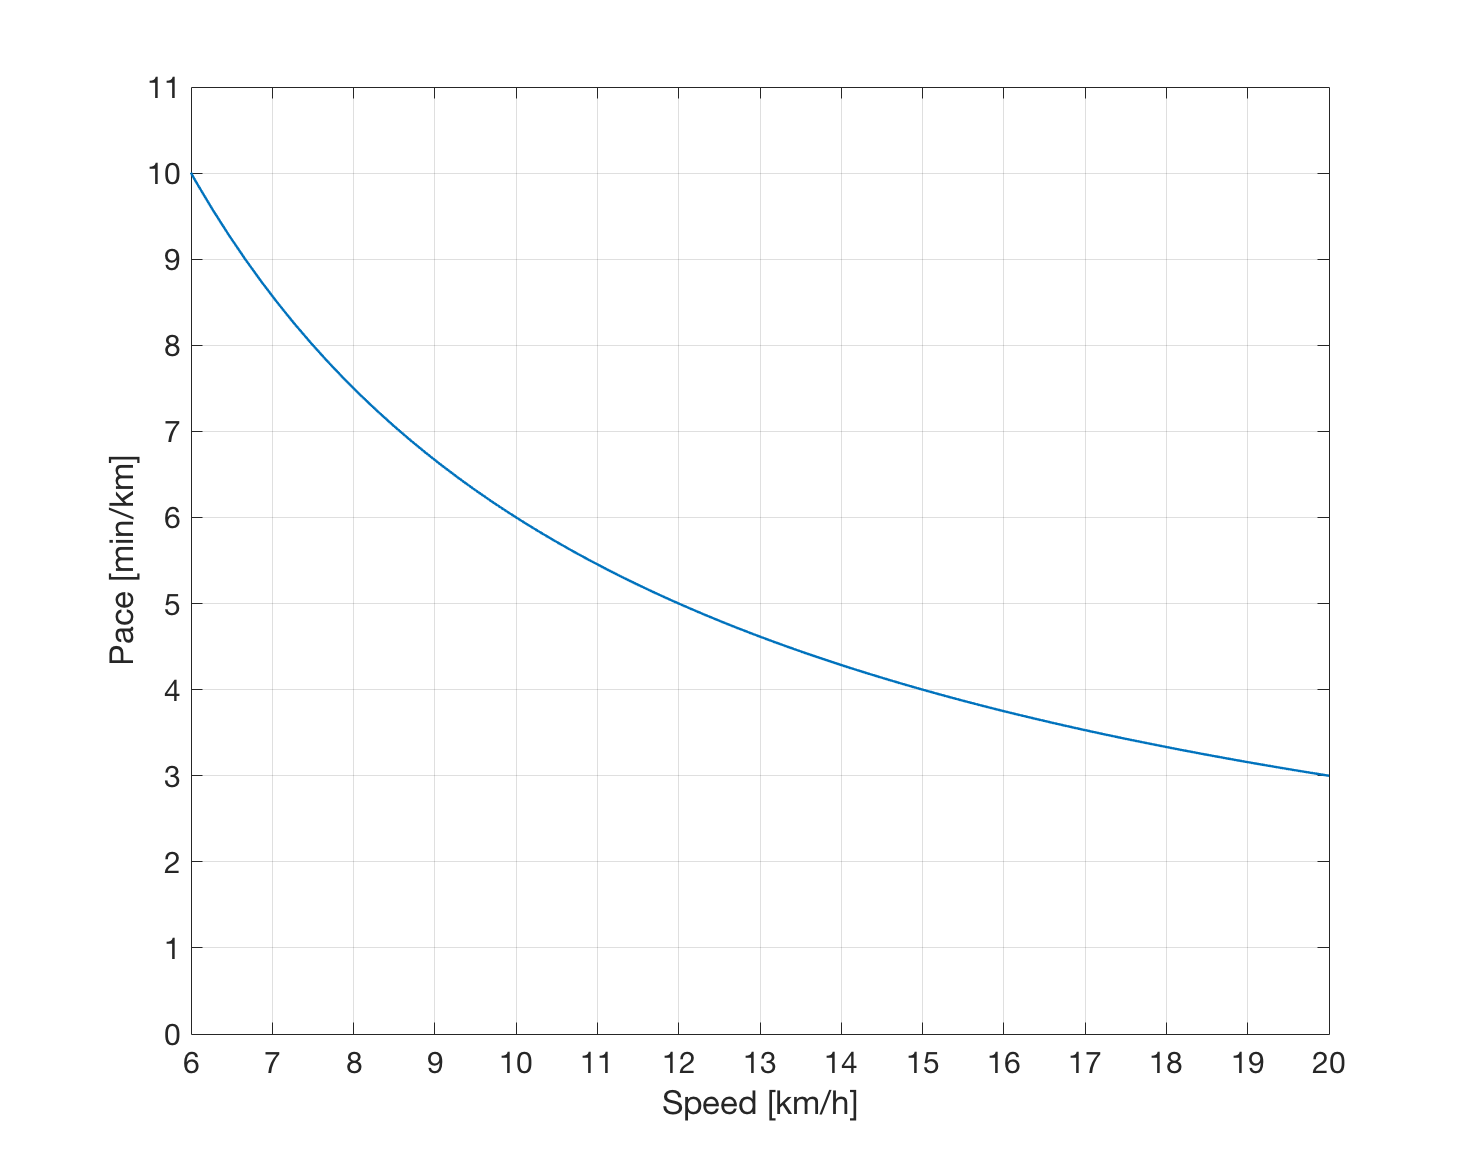
\includegraphics[width=0.8\linewidth]{Figures/PacevsSpeed.png}
	\caption{This is a figure of format PNG of dimensions 1468 x 1162 pixels. The caption is in italic with a bold title. The figure width is 0.8 of the linewidth (textwidth). Height is scaled to keep original proportions.}
	\label{Fig:}
\end{figure}

\lipsum[1]

\subsection{Blocks of (sub)figures}

\begin{figure}[H]
  \begin{minipage}[b]{.5\linewidth}
    \centering
	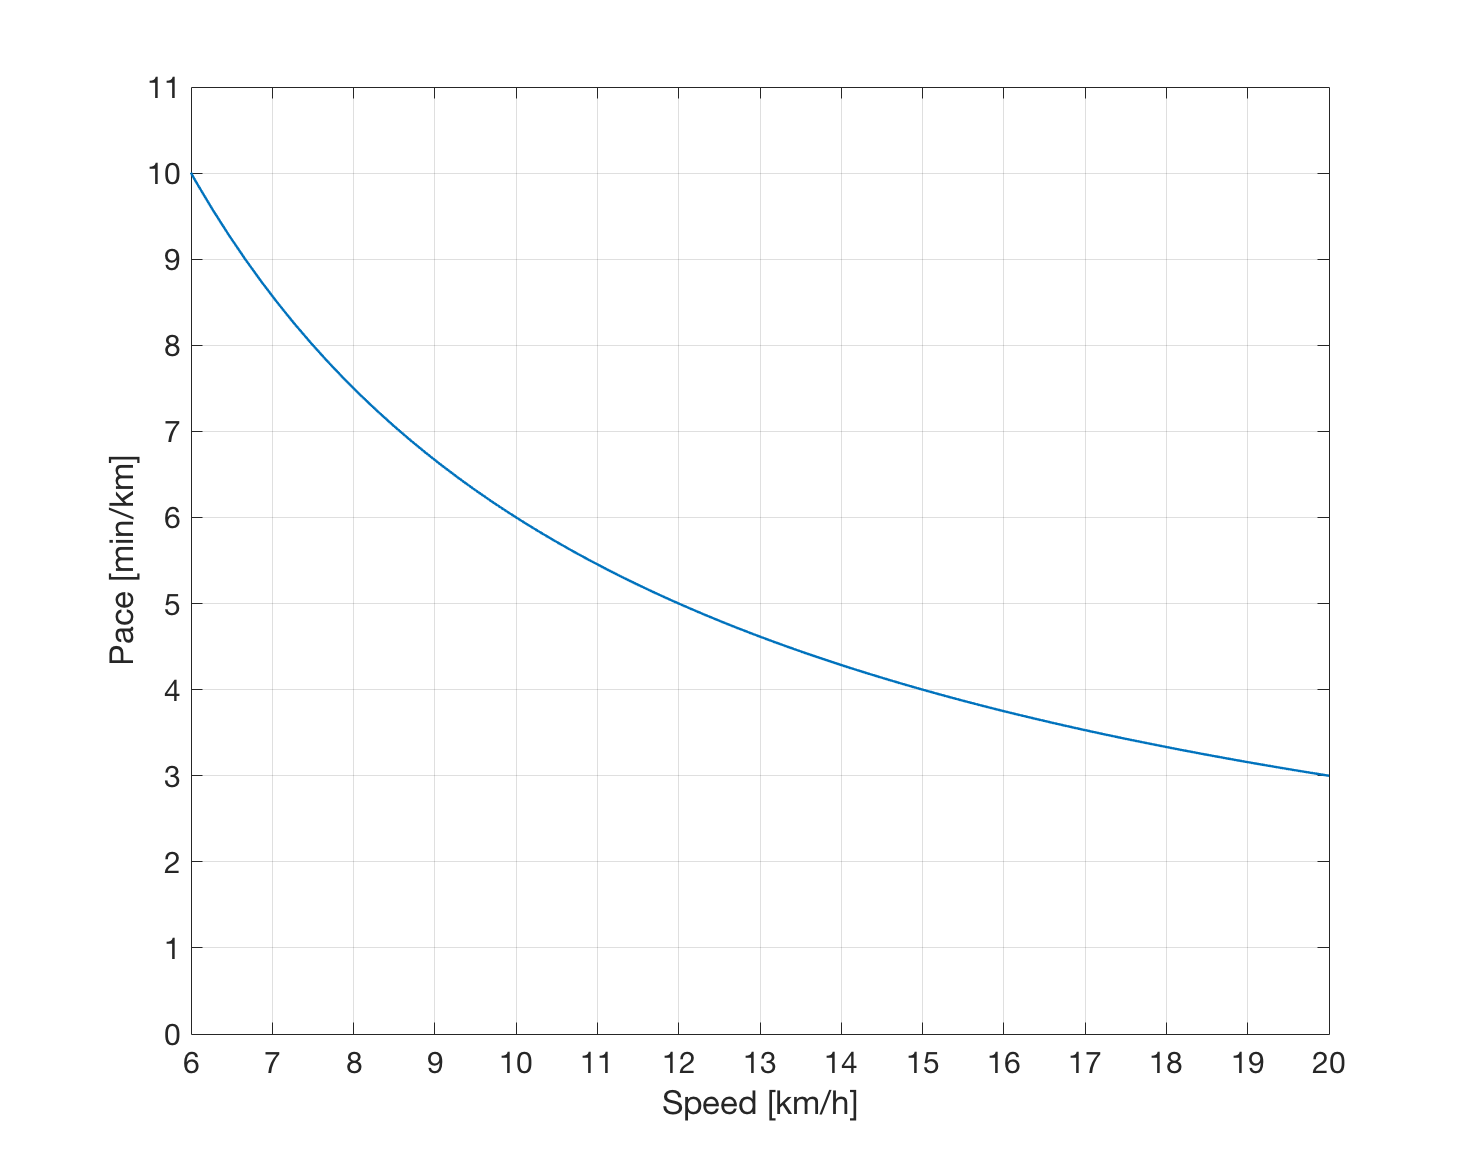
\includegraphics[width=0.8\linewidth]{Figures/PacevsSpeed.png}
    \caption{This is a subfigure.}
	\label{fig:1a}
  \end{minipage}%
  \begin{minipage}[b]{.5\linewidth}
    \centering
	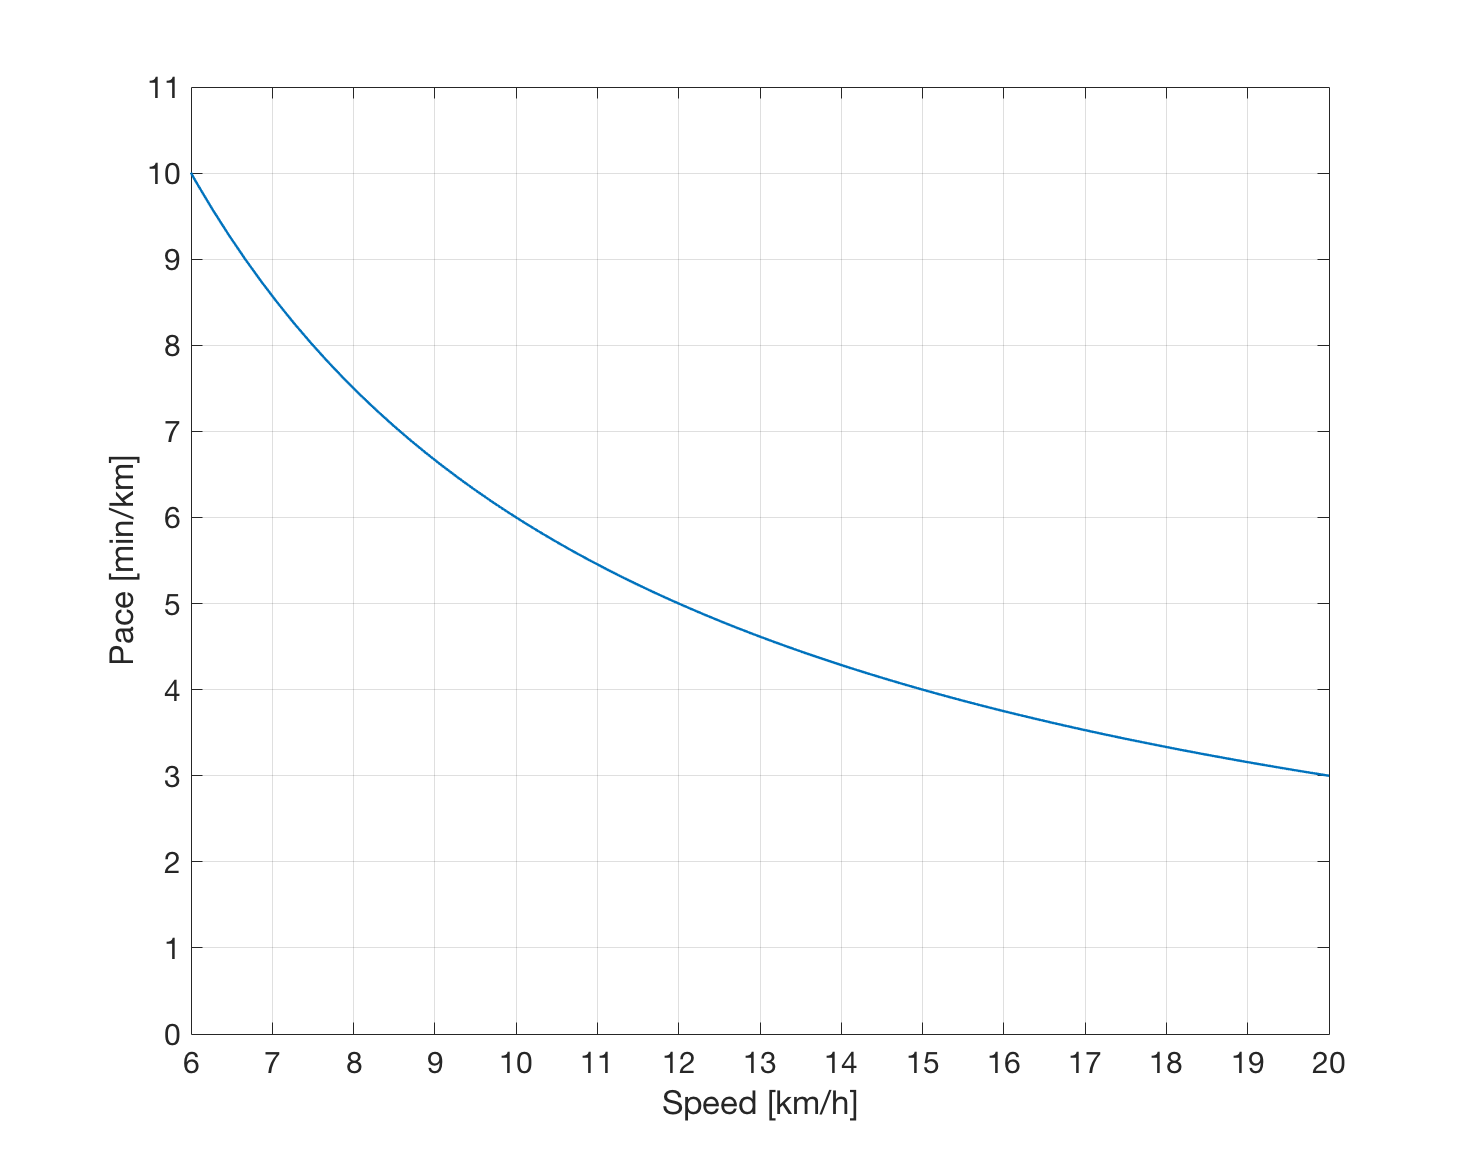
\includegraphics[width=0.8\linewidth]{Figures/PacevsSpeed.png}
    \caption{And this is another subfigure.}
	\label{fig:1b}
  \end{minipage}
  \label{fig:1}
\end{figure}



\lipsum[1]

\begin{figure}[H]
  \begin{minipage}[b]{.5\linewidth}
    \centering
	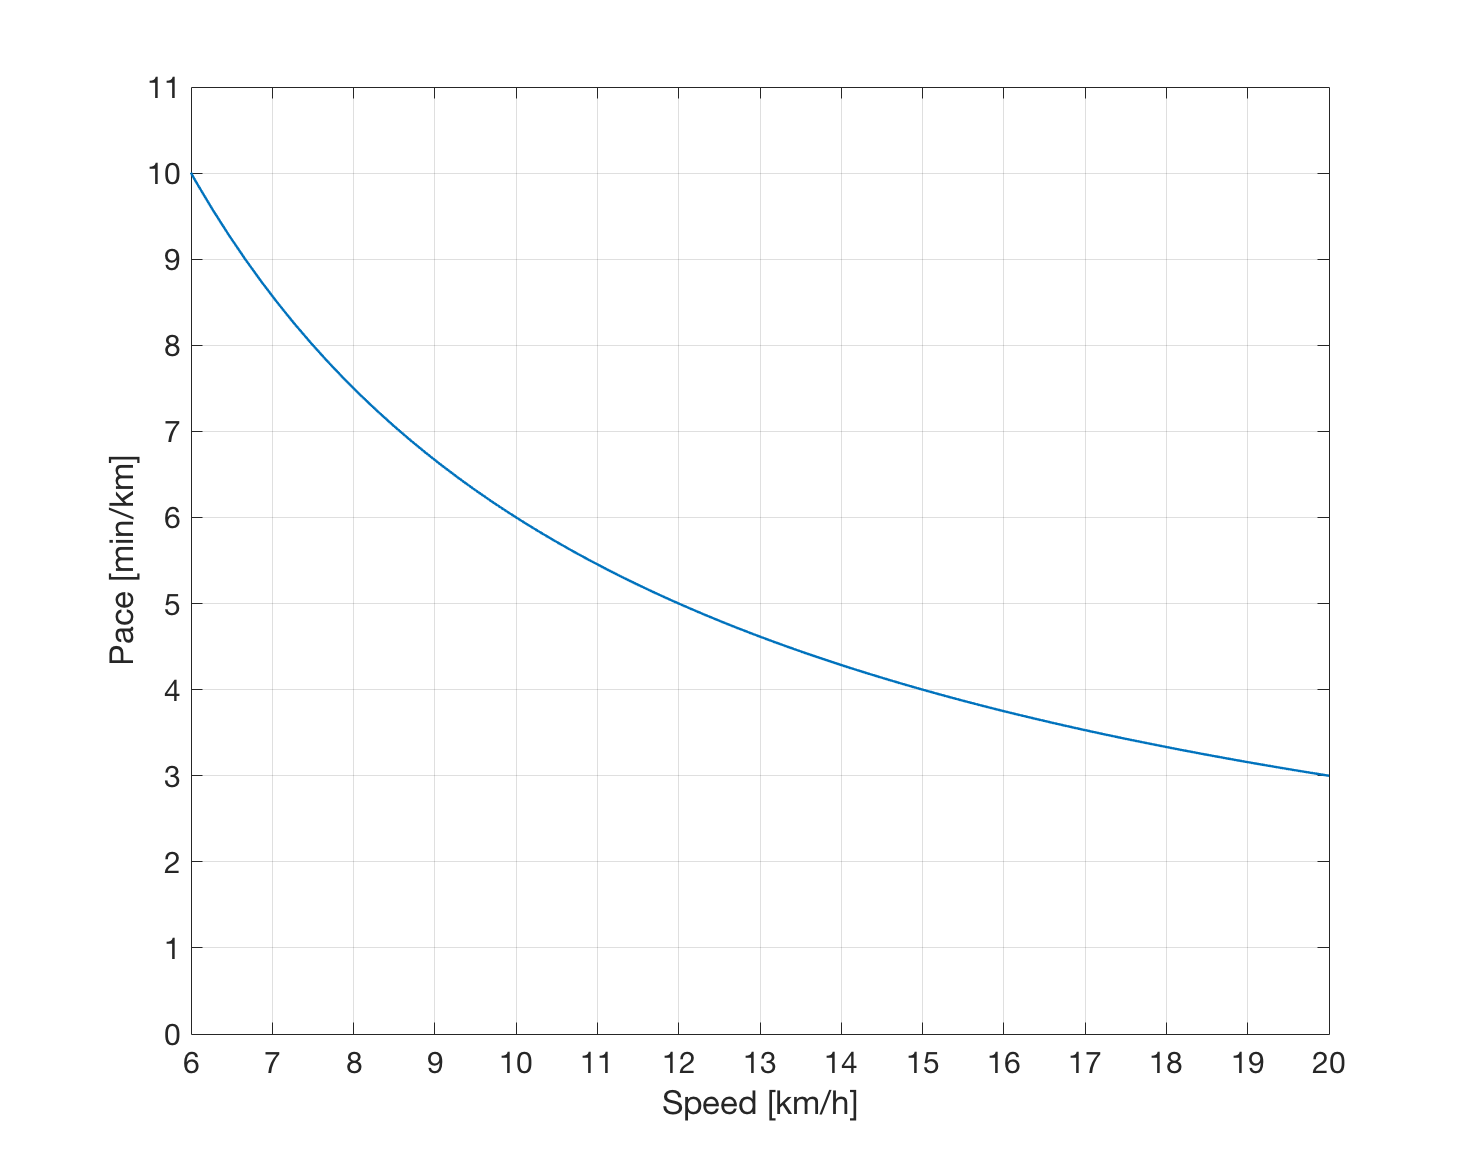
\includegraphics[width=0.8\linewidth]{Figures/PacevsSpeed.png}
    \subcaption{This is a subfigure.}
	\label{fig:1a}
  \end{minipage}%
  \begin{minipage}[b]{.5\linewidth}
    \centering
	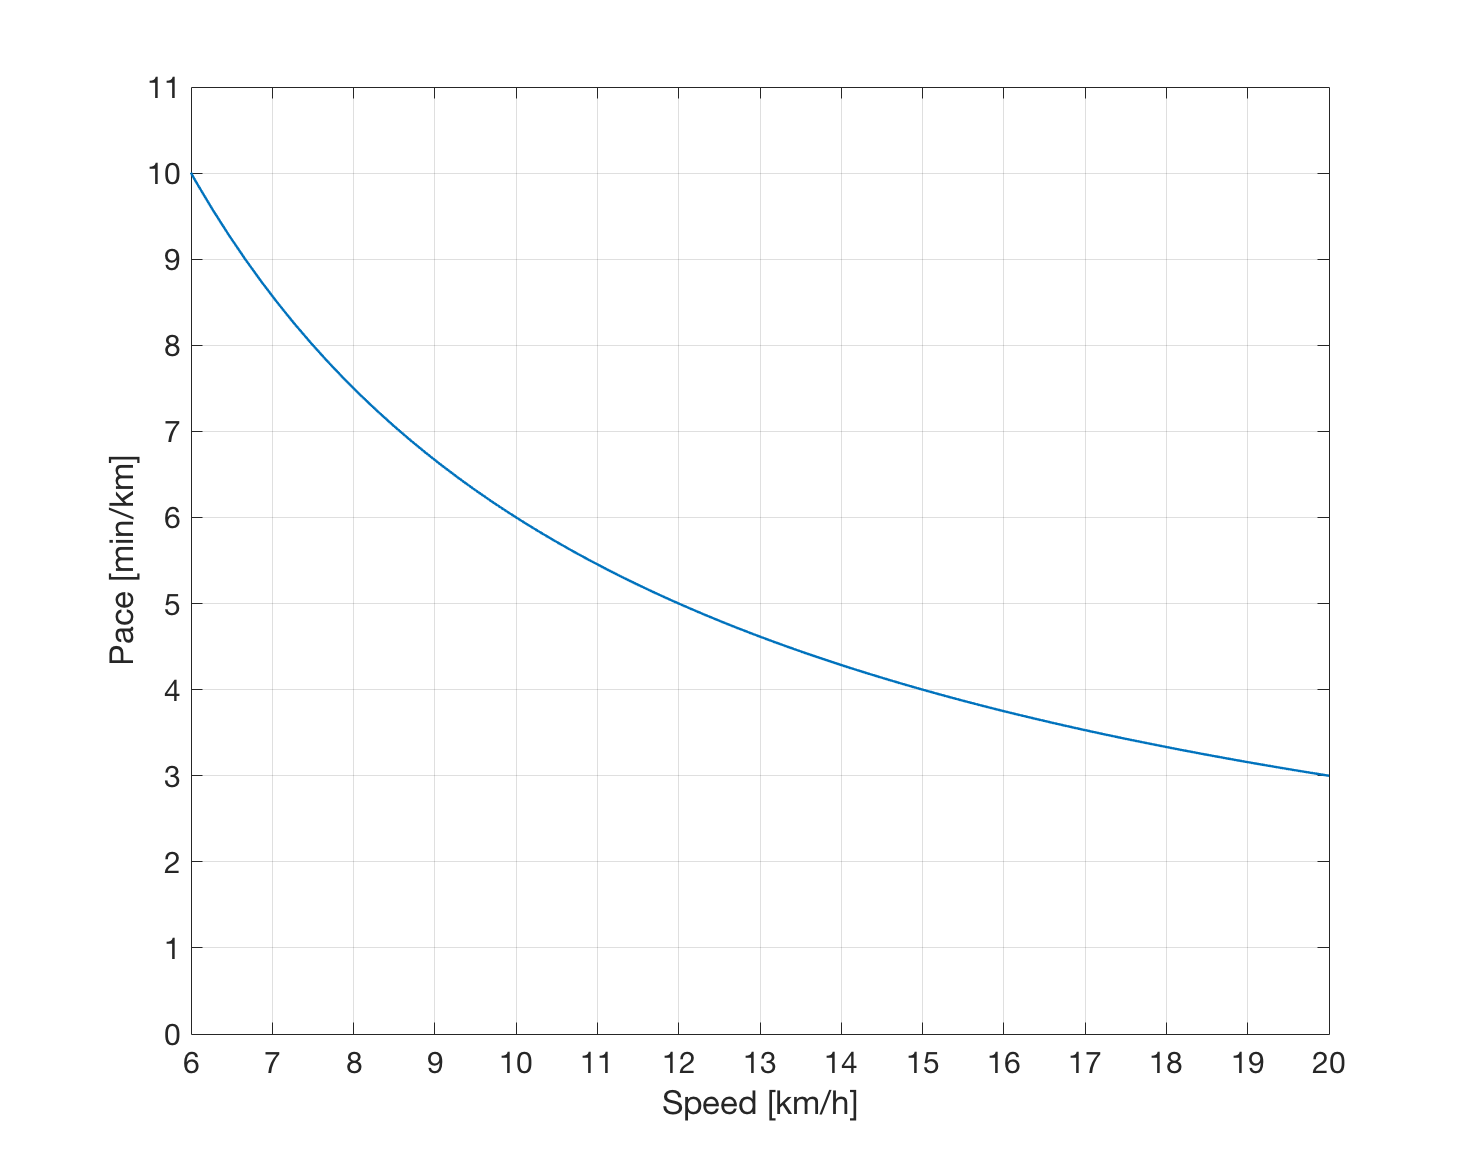
\includegraphics[width=0.8\linewidth]{Figures/PacevsSpeed.png}
    \subcaption{And this is another subfigure.}
	\label{fig:1b}
  \end{minipage}
  \label{fig:1}
  \begin{minipage}[b]{.5\linewidth}
    \centering
	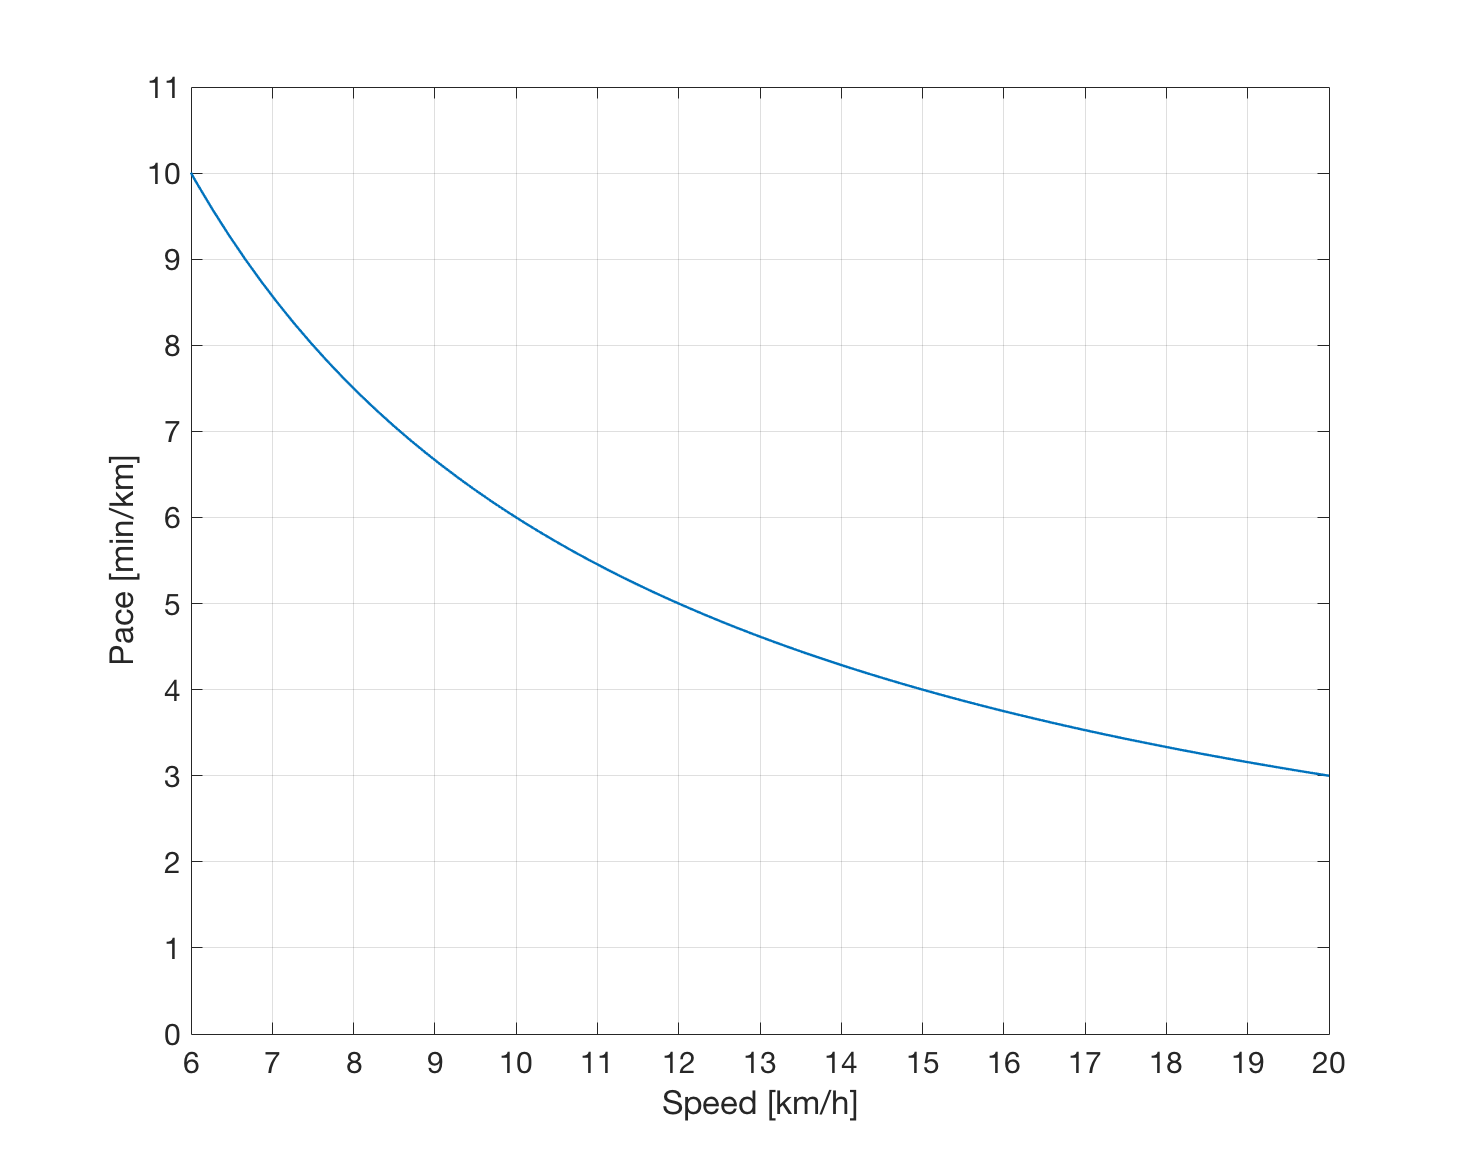
\includegraphics[width=0.8\linewidth]{Figures/PacevsSpeed.png}
    \subcaption{And this is another subfigure.}
	\label{fig:1a}
  \end{minipage}%
  \begin{minipage}[b]{.5\linewidth}
    \centering
	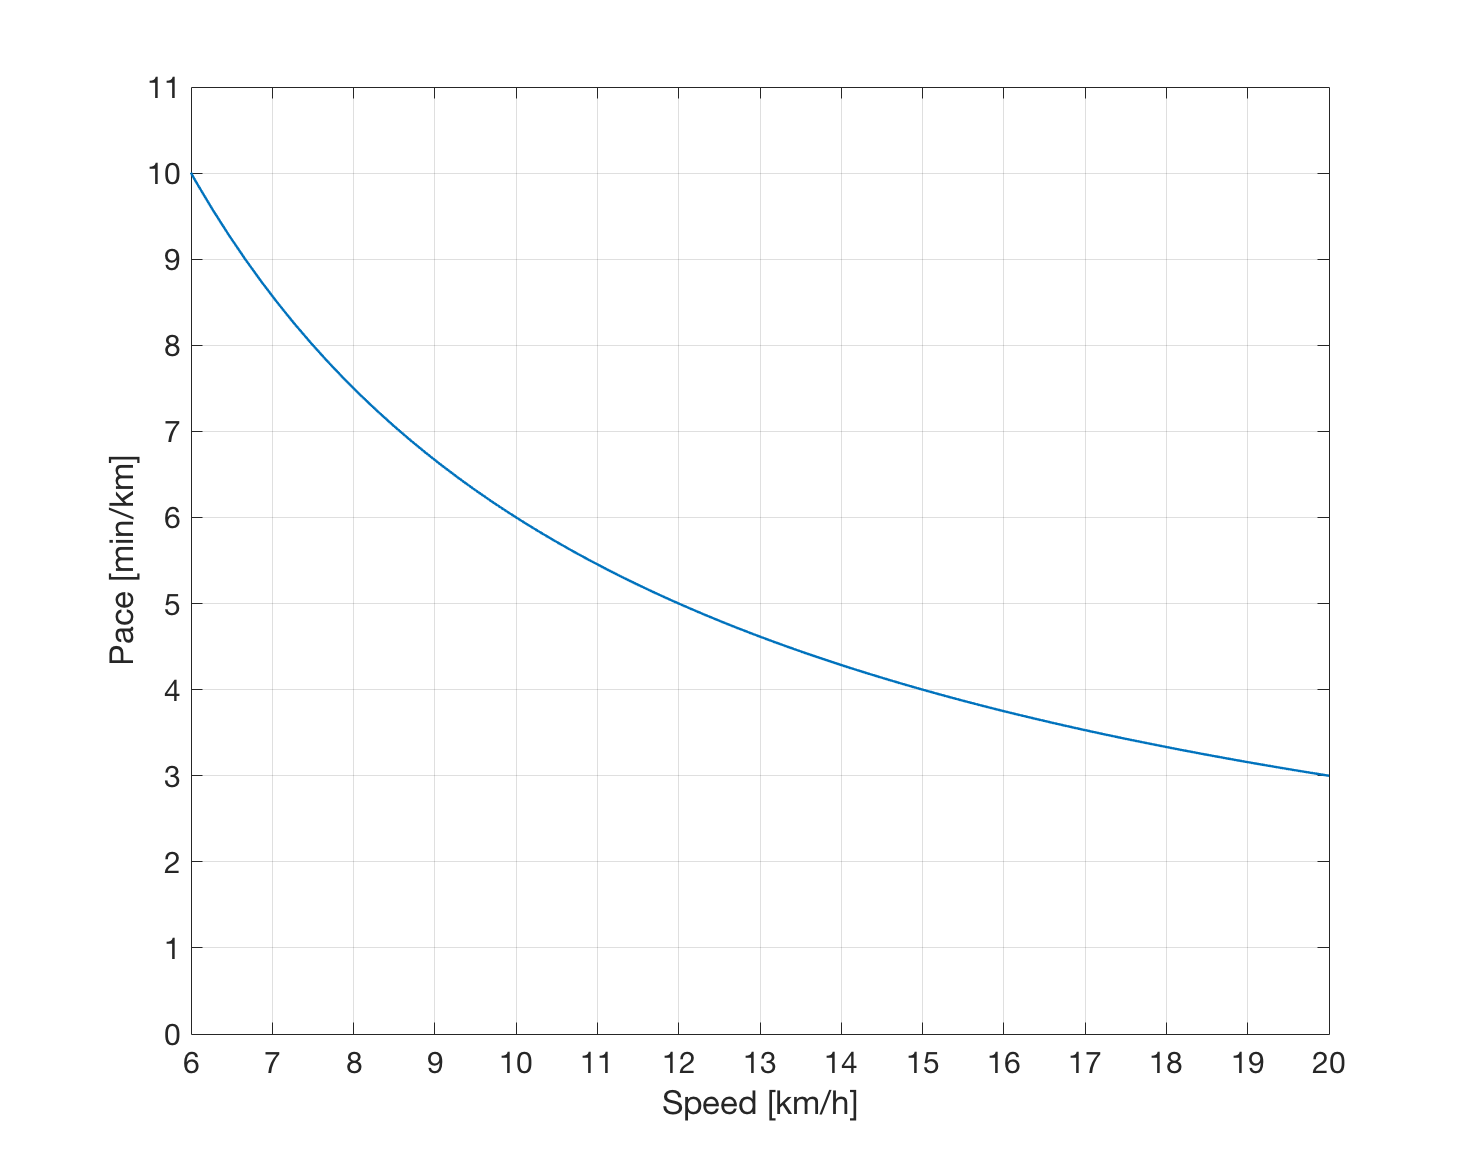
\includegraphics[width=0.8\linewidth]{Figures/PacevsSpeed.png}
    \subcaption{And this is another subfigure.}
	\label{fig:1b}
  \end{minipage}
  \caption{This is the figure with subfigures.}
  \label{fig:1}
\end{figure}

\subsection{Wrapped figure}

\begin{wrapfigure}{r}[0pt]{0.5\linewidth}
	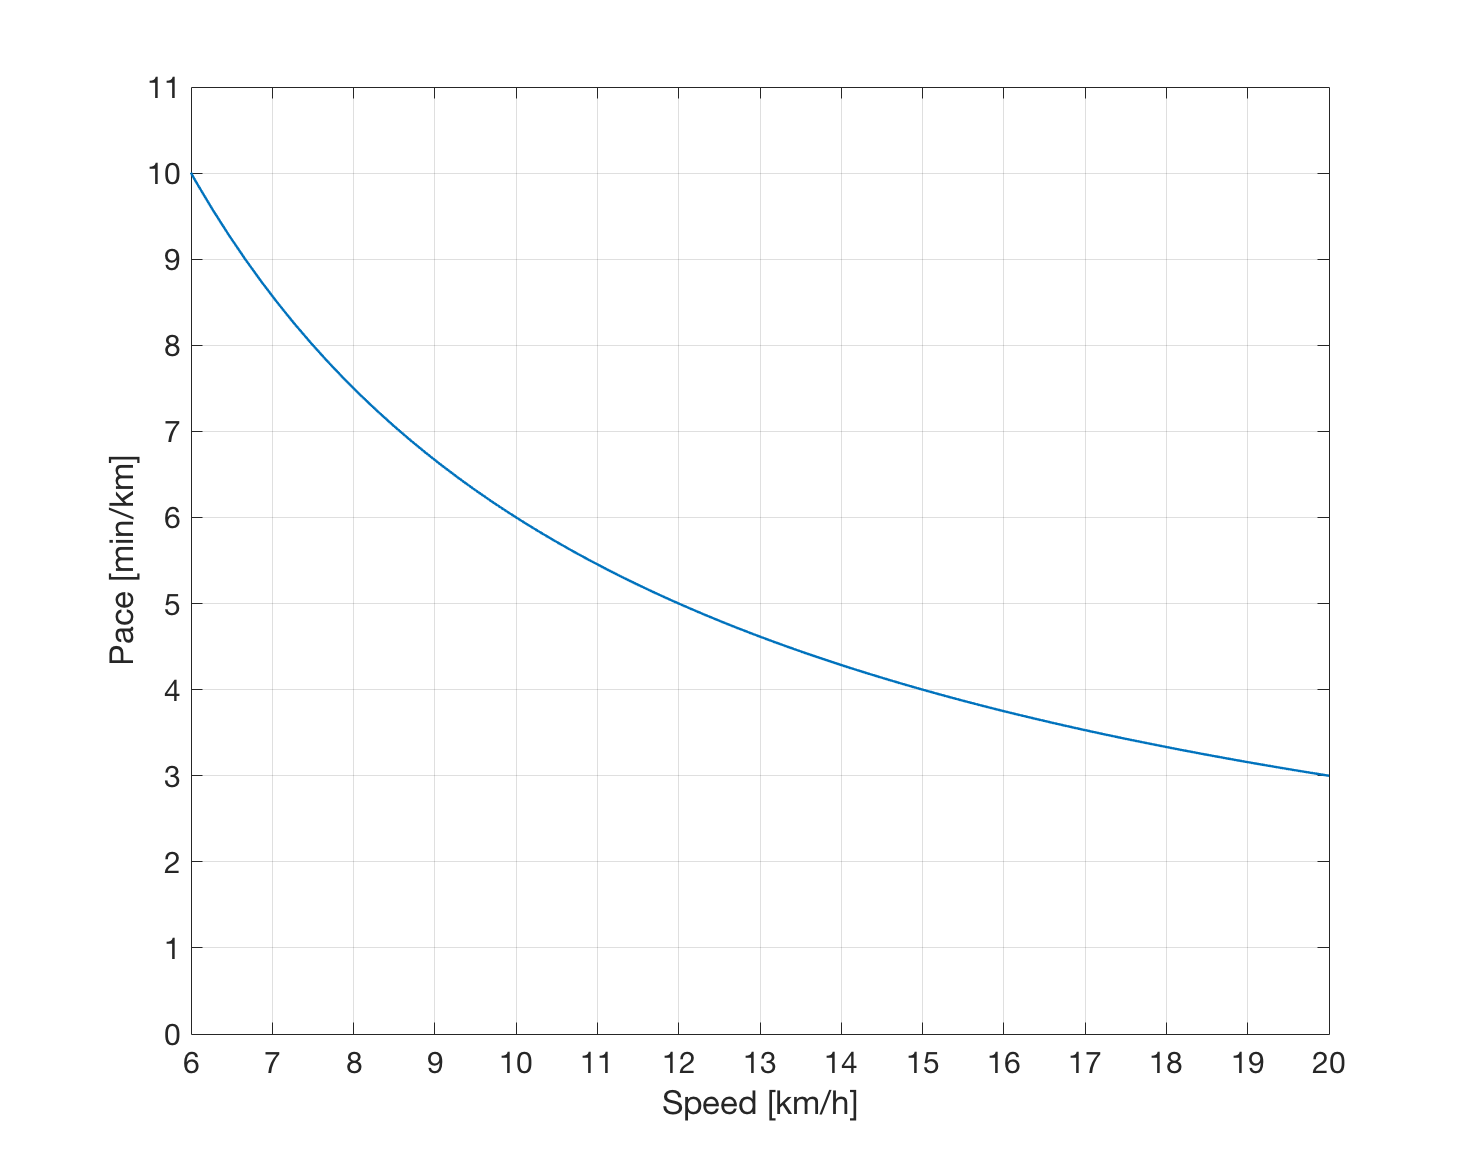
\includegraphics[width=\linewidth]{Figures/PacevsSpeed.png}
	\caption{This figure is wrapped in the text.}
	\label{Fig:}
\end{wrapfigure}

\lipsum[1-2]



%\input{Introduction}
% or
\section{Headers and footers}
\lipsum[1-2]\cite{latexcompanion}

%\input{Theory}
% or
\section{Theory}
\lipsum[1-3]\cite{knuthwebsite}
%\input{Method}
% or
\section{Method}
\lipsum[1-2]
%\input{Results}
% or
\section{Results}
\lstinputlisting{Problem1919.py}

%\input{Discussion}
% or
%\section{Discussion}

\begin{thebibliography}{3}
\bibitem{latexcompanion}
Michel Goossens, Frank Mittelbach, and Alexander Samarin.
\textit{The \LaTeX\ Companion}.
Addison-Wesley, Reading, Massachusetts, 1993.

\bibitem{einstein}
Albert Einstein.
\textit{Zur Elektrodynamik bewegter K{\"o}rper}. (German)
[\textit{On the electrodynamics of moving bodies}].
Annalen der Physik, 322(10):891–921, 1905.

\bibitem{knuthwebsite}
Knuth: Computers and Typesetting,
\\\texttt{http://www-cs-faculty.stanford.edu/\~{}uno/abcde.html}
\end{thebibliography}

% -------------------------------------------------------------KOMMENTAR/FILIP
\begin{appendices}
    \section{Lorem}
    \begin{figure}[H]
    	\centering
    	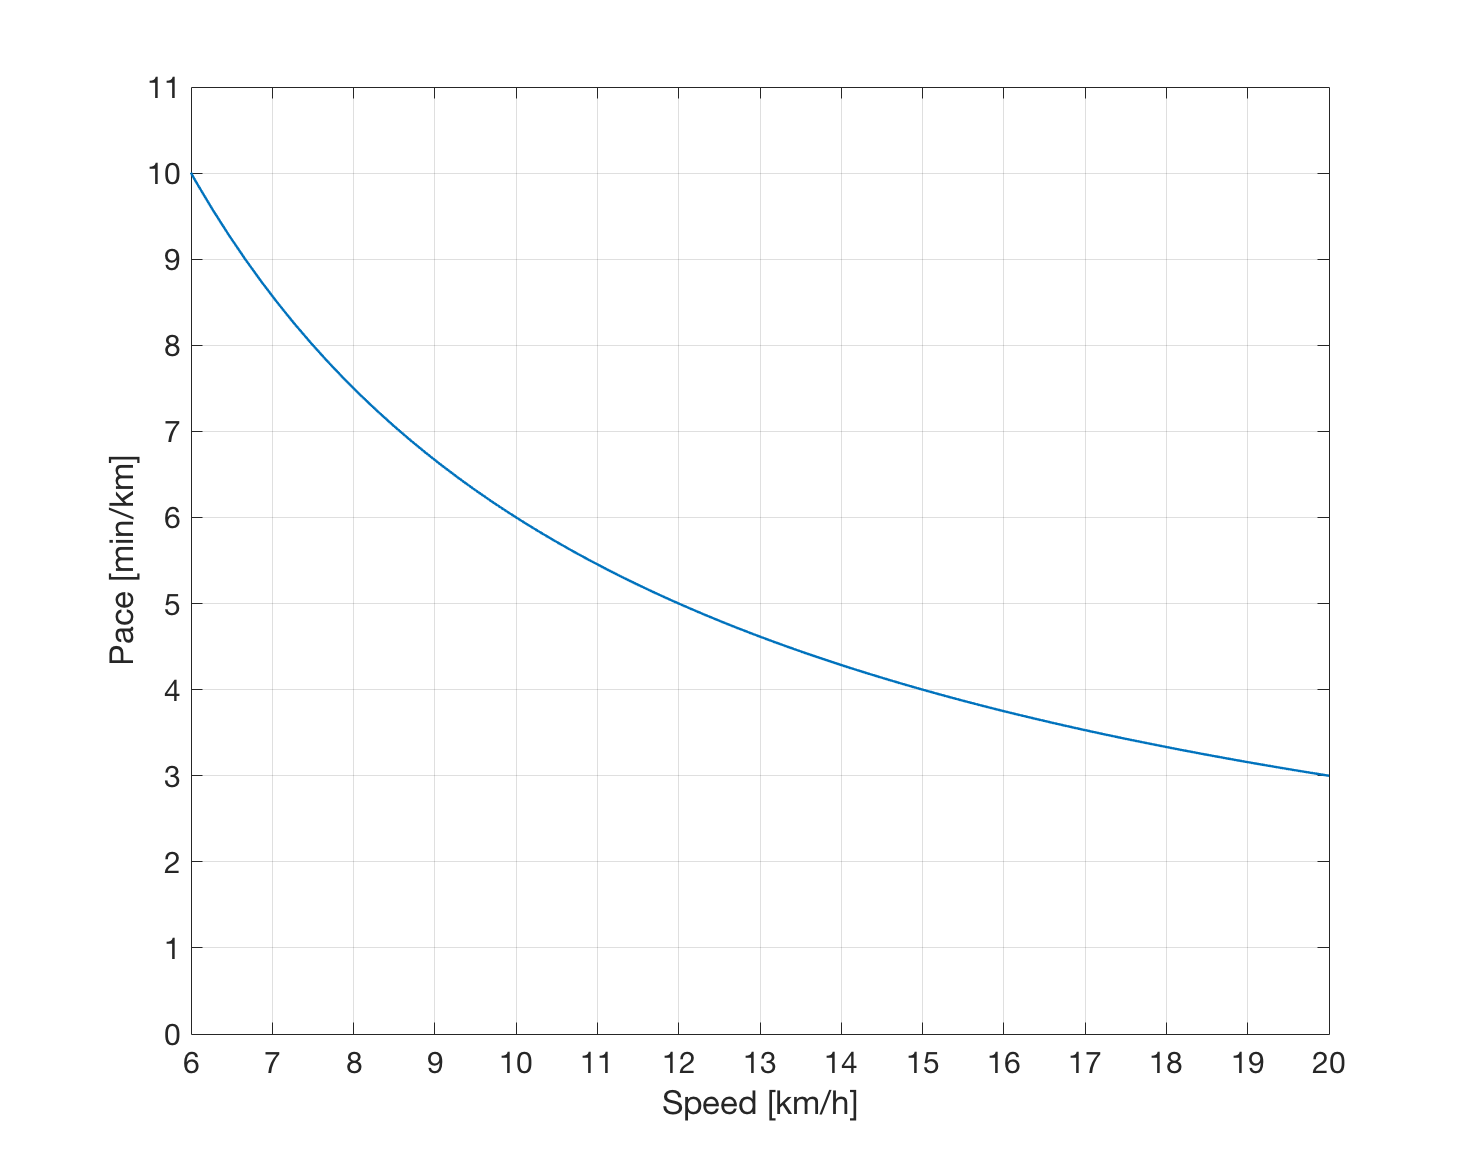
\includegraphics[width=0.8\linewidth]{Figures/PacevsSpeed.png}
    	\caption{This is a figure of format PNG of dimensions 1468 x 1162 pixels. The caption is in italic with a bold title. The figure width is 0.8 of the linewidth (textwidth). Height is scaled to keep original proportions.}
    	\label{Fig:}
    \end{figure}
    \section{Ipsum}
    \lipsum[2]
    \section{Dolor}
    \lipsum[3]
\end{appendices}

\end{document}
% -------------------------------- End Document -------------------------------
